\documentclass[letterpaper,10pt]{article}
\usepackage{standalone}
\usepackage[spanish]{babel}
\usepackage[utf8]{inputenc}
\usepackage{ragged2e}
\usepackage{graphicx}
\usepackage[binary-units]{siunitx}
\usepackage{amsthm}% http://ctan.org/pkg/amsthm
\usepackage[left=2.5cm, top=2.5cm, right=2.5cm, bottom=3cm]{geometry}
\usepackage{lastpage}
\usepackage{fancyhdr}
\usepackage{listings}
\usepackage{multicol}
\usepackage{hyperref}
\usepackage{color}
\usepackage{placeins}
\definecolor{aliceblue}{rgb}{0.94, 0.97, 1.0}
\definecolor{mygreen}{rgb}{0.40, 0.67, 0.3}
\definecolor{antiquewhite}{rgb}{0.98, 0.92, 0.84}
\usepackage{pgfplots}
\pgfplotsset{compat=newest}
%% the following commands are needed for some matlab2tikz features
\usetikzlibrary{plotmarks}
\usetikzlibrary{arrows.meta}
\usepgfplotslibrary{patchplots}
\usepackage{grffile}
\usepackage{amsmath}

\usepackage{listings}
\usepackage{lstautogobble} % Fix relative indenting
\renewcommand{\lstlistingname}{Listado}
\lstset{
	backgroundcolor={\color{white}},basicstyle={\small \ttfamily},breaklines=true,captionpos=b,commentstyle={\color{mygreen}},emph={[1]{for,end,break}},emphstyle={[1]\color{red}},frame=tb,identifierstyle={\color{black}},keywordstyle={\color{blue}},language=Matlab,morekeywords={[2]{1}},numbers=left,numbersep=9pt,numberstyle={\tiny \color{black}},showstringspaces=false,stringstyle={\color{red}}}
\usepackage[shortlabels]{enumitem}

\pagestyle{fancy}
\renewcommand{\headrulewidth}{0pt}
\fancyhf{}% clear all fields
\fancyfoot[C]{\thepage\ de \pageref{LastPage}}

\setlength{\parskip}{3pt}

\begin{document}	
\begin{titlepage}
	\begin{figure}[h!]
		\begin{center}
			\vspace{1.5cm}
			% Aquí se inserta un escudo o emblema:
			
\includegraphics[scale= .5, ]{encabezado.png}
			\label{escudouam1}
			\vspace{-1cm}
		\end{center}
	\end{figure}
	\begin{center}
		\vspace{1cm} 
		\LARGE{\textbf{INSTITUTO TECNOLÓGICO DE MORELIA}} \\
		\vspace{1cm}
		DEPARTAMENTO DE INGENIERÍA ELECTRÓNICA
		DIVISIÓN DE ESTUDIOS PROFESIONALES \\  
		%nombre del prof
		\vspace{2.3cm} {\large \textbf{MATERIA}\\ \LARGE CONTROL 1}
		
		% Incrementamos el interlineado
		%TEMA
		
		\vspace{1.5cm} {\large \textbf{REPORTE DE LABORATORIO}\\ \LARGE Poles and zeros found by inspection}\\ 
		
		\vspace{1.5cm} {\large \textbf{PROFESOR}\\ \LARGE GERARDO MARX CHÁVEZ CAMPOS}
		
		\vspace{1.5cm} {\large \textbf{ALUMNOS}\\ \large JORGE ALBERTO OCHOA LÓPEZ\\JOSÉ EDUARDO CONTRERAS SANDOVAL} \\
		\normalsize{7º semestre
			%fecha
			\hfill {24/11/17}}\\ 
		MORELIA, MICHOACÁN
	\end{center}
\end{titlepage}
\pagebreak
\justify
\tableofcontents
\pagebreak
\pagenumbering{arabic}
	
	\section{INTRODUCCION:} El objetivo principal de esta práctica es analizar un circuito sencillo, en el cual debemos de obtener su función de transferencia por el método de inspección y algebraicamente, esto con la finalidad de poder obtener la respuesta del sistema mediante una función realizada en la práctica pasada donde obteníamos una gráfica de la respuesta de un sistema dado. Después simulamos el circuito con valores reales de resistencias y de un inductor para obtener la gráfica de Bode la cual nos da el comportamiento del sistema en el dominio de la frecuencia, finalmente hicimos la implementación física del circuito y medimos los voltajes de salida para obtener nuestra gráfica de Bode real. \\
	
	Para la primer parte de la práctica nos piden obtener la función de transferencia del circuito dado, con el método de inspección se hace un análisis de corriente directa donde el inductor se comporta como un corto, de esta forma podemos calcular el término $G_{0}$ el cual está dado por la siguiente equivalencia:
	\[G_{0}=\frac{V_{out}(s)}{V_{in}(s)}\]
	Después tenemos que buscar la rama del circuito que nos afecte el voltaje de salida al presentarse una variación en la frecuencia para de esta manera poder identificar los polos y los ceros para finalmente obtener la función de transferencia, la cual la sustituiremos por los valores de los componentes utilizados para poder obtener una gráfica de la respuesta del sistema mediante el código previamente realizado.\\
	
	En la segunda parte basicamente solo simulamos el circuito para de igual forma ver su respuesta. Finalmente hicimos la implementación del circuito para medir con el osciloscopio la respuesta real de nuestro sistema y poder compararlo con lo obtenido teóricamente y en la simulación.\\
	\section{METODOLOGIA:}
	\subsection{Parte 1} 
	\textbullet Obtener la función de transferencia por inspección del siguiente circuito.\\
	
	\textbullet Obtener la función de transferencia utilizando técnicas comunes de álgebra.\\
	
	\textbullet Usando la función desarrollada en Scilab o Matlab checar la respuesta.
	\begin{figure}[h!]
		\centering
		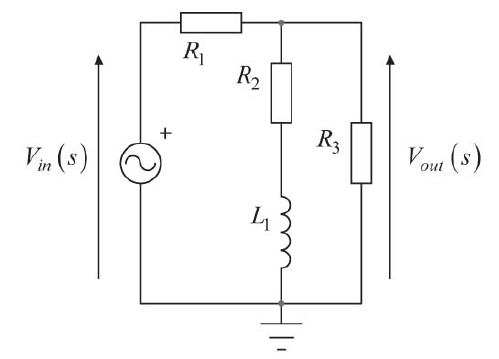
\includegraphics[width=0.5\linewidth]{circuito_1}
		\caption{Circuito para la parte 1.}
		\label{fig:circuito1}
	\end{figure}
\FloatBarrier
Para el método de inspección lo primero que se tiene que realizar es hacer el análisis de corriente directa para obtener el término $G_{0}$ donde el inductor se comporta como un corto circuito por lo que el circuito queda de la siguiente forma:
\begin{figure}[h!]
	\centering
	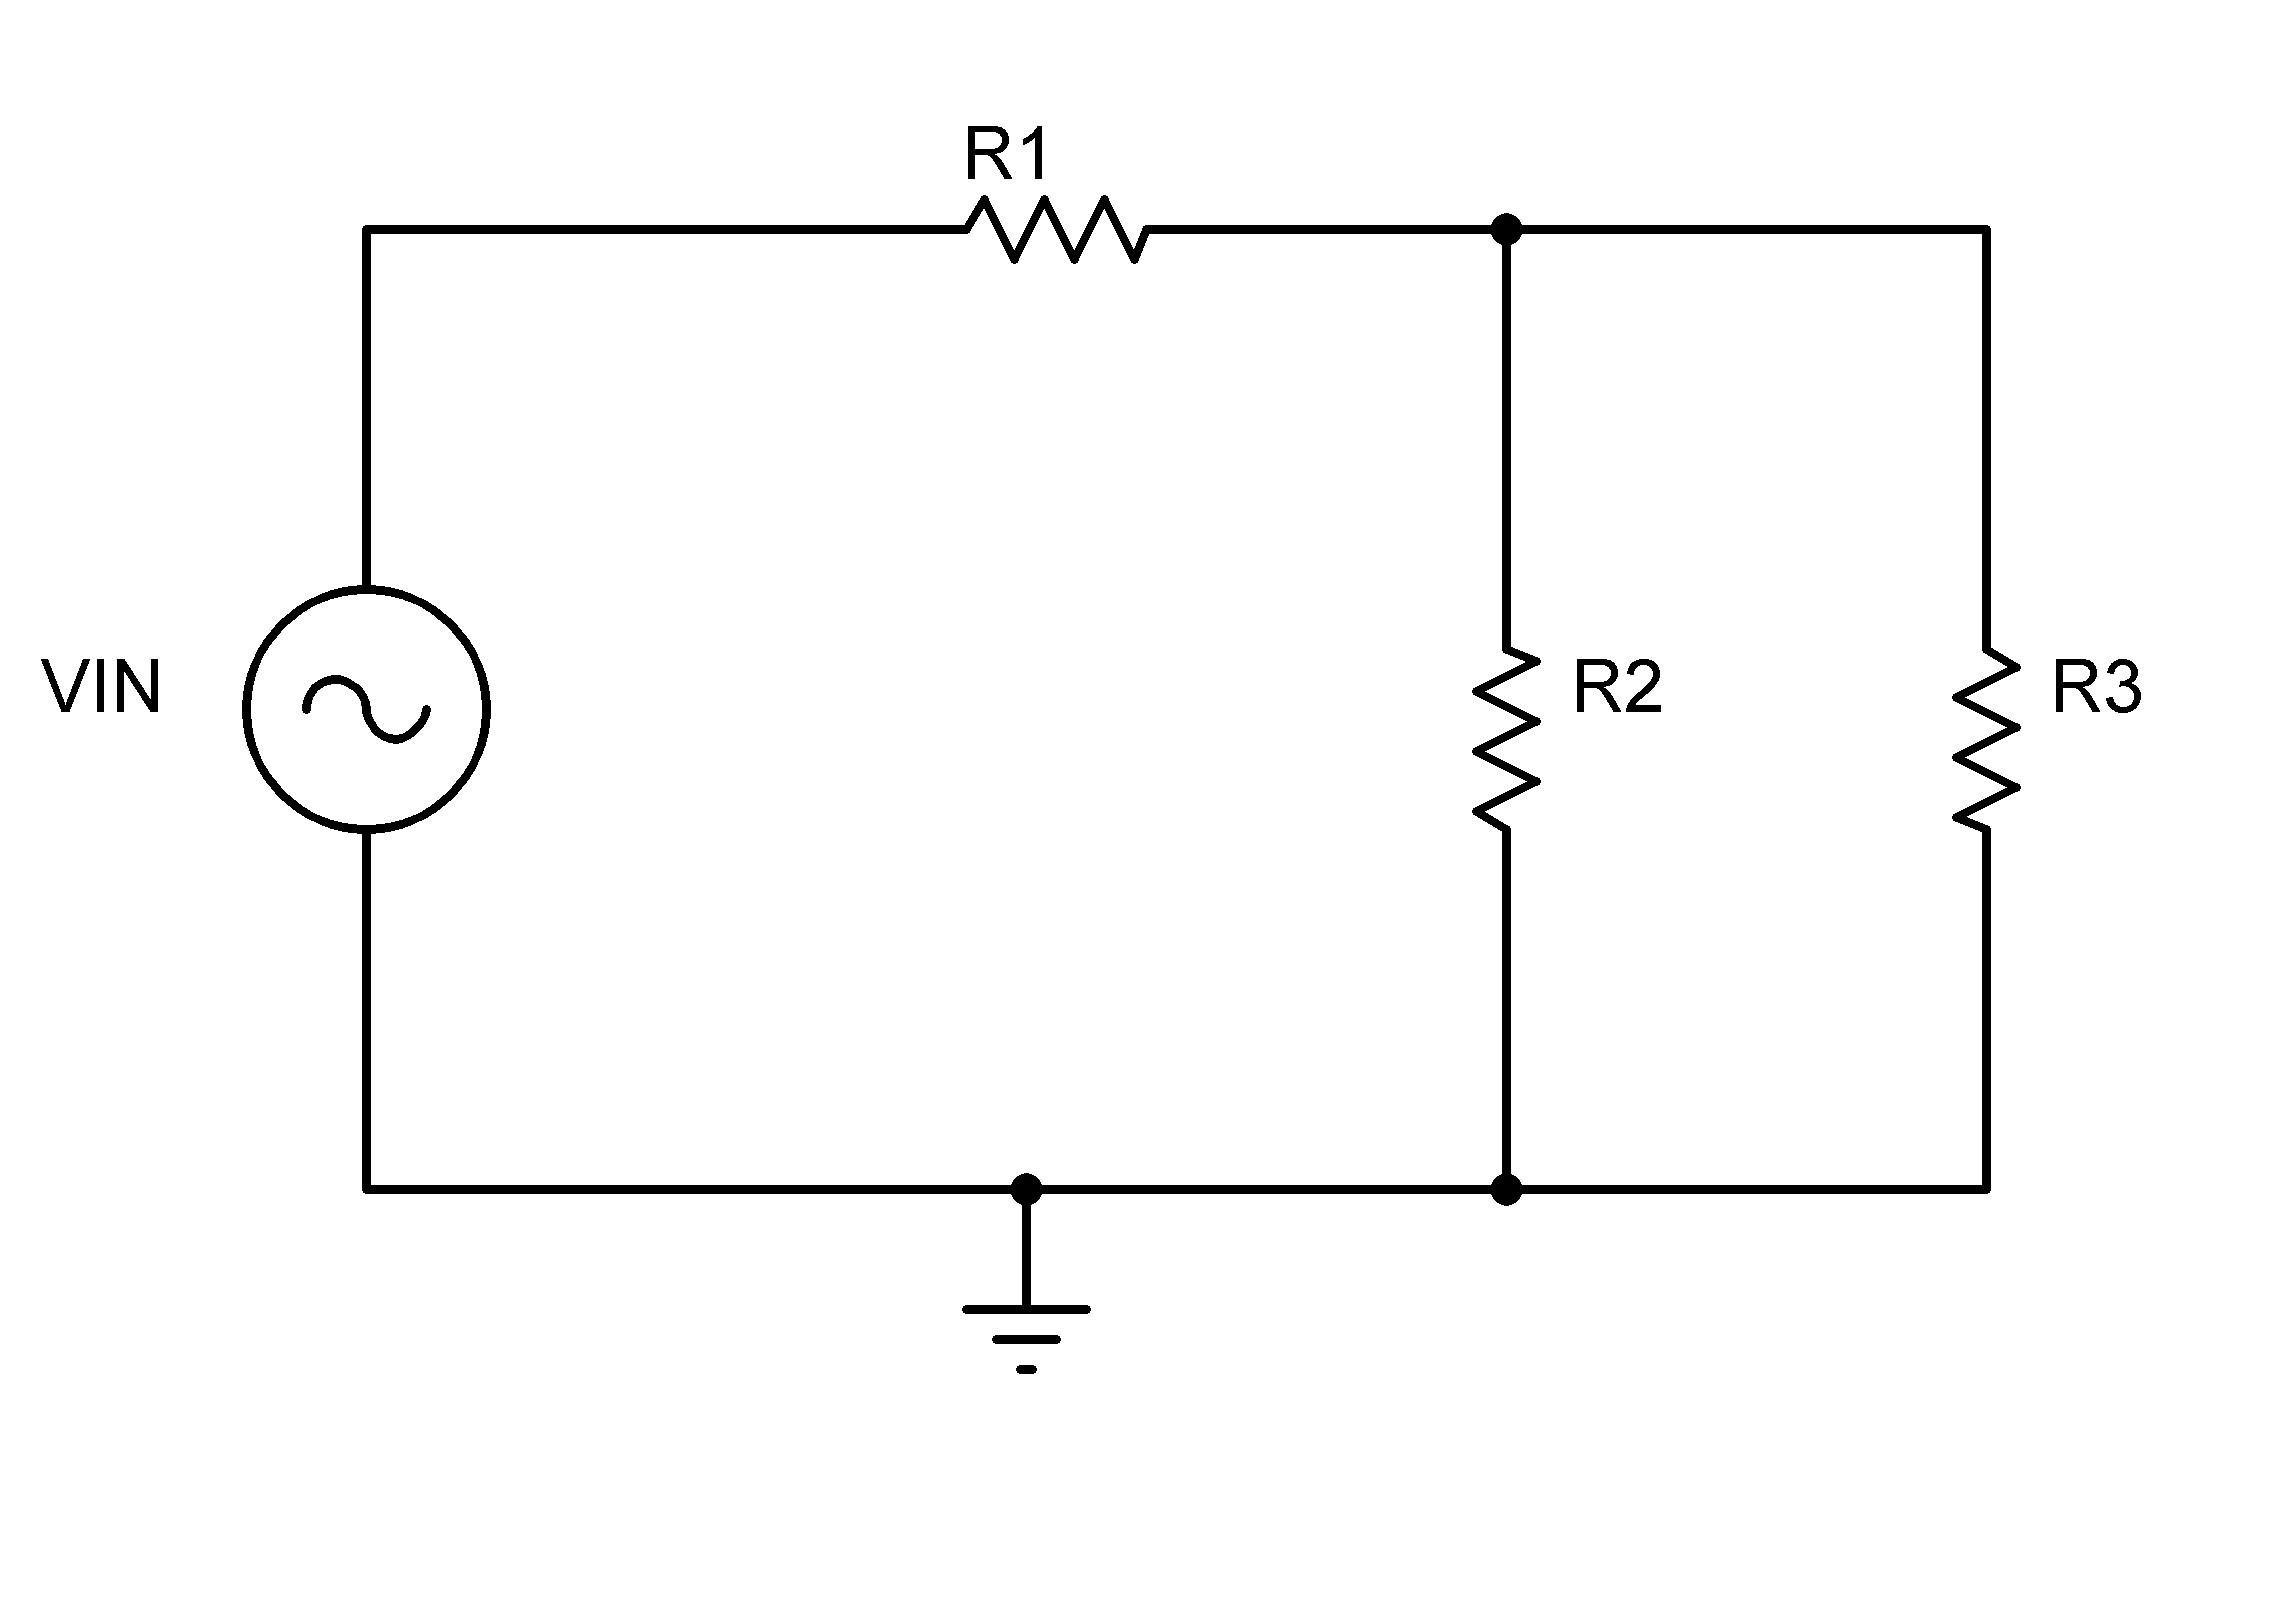
\includegraphics[width=0.5\linewidth]{esque_1}
	\caption{Circuito resultante al hacer el análisis en corriente directa}
	\label{fig:esque1}
\end{figure}
\FloatBarrier
Lo siguiente que se realiza es hacer un divisor de voltaje para obtener el voltaje de salida del circuito de la figura \ref{fig:esque1} 
\[V_{out}(s)=V_{in}\frac{R2||R3}{R1+(R2||R3)}\]
Se pasa $V_{in}$ del otro lado para obtener $G_{0}$.
\[G_{0}=\frac{V_{out}(s)}{V_{in}(s)}=\frac{R2||R3}{R1+(R2||R3)}\]
Para obtener los ceros se tiene que identificar la rama del circuito que nos afecte el voltaje de salida al variar la frecuencia la cual es la rama donde está el inductor.
\[R2+J\omega L=0\]
\[1+\frac{SL}{R2}=0\]
\[\frac{1}{\omega_{z1}}=\frac{L}{R2}\]
\[\omega_{z1}=\frac{R2}{L}\]
Para obtener los polos las fuentes de voltaje se ponen en corto circuito por lo que el circuito queda de la siguiente forma:
\begin{figure}[h!]
	\centering
	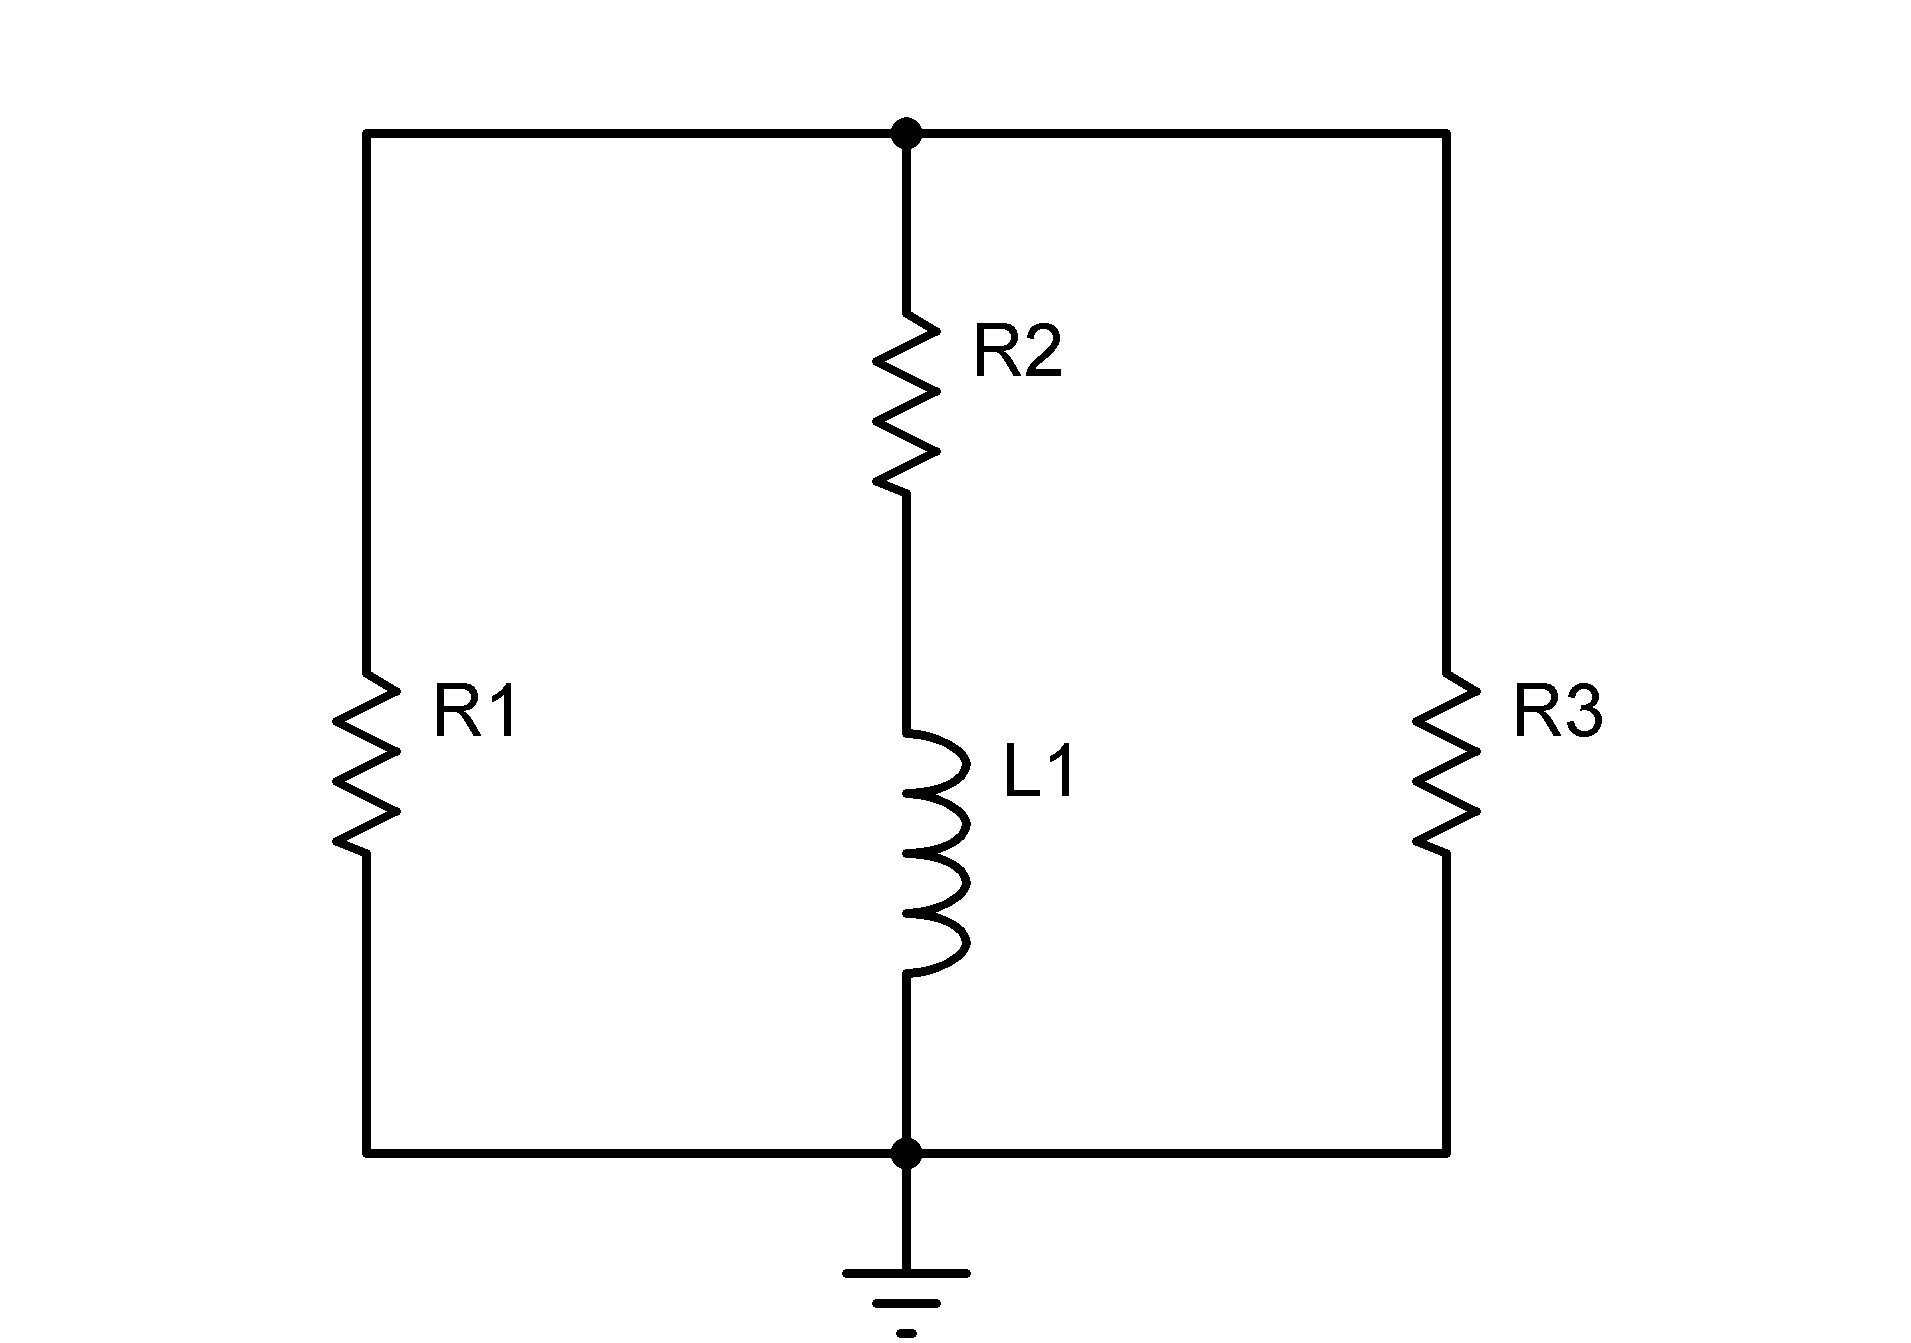
\includegraphics[width=0.5\linewidth]{esque_2}
	\caption{Circuito resultante al poner en corto la fuente de voltaje.}
	\label{fig:esque2}
\end{figure}
\FloatBarrier
Del circuito anterior se obtienen los polos quedando de la siguiente manera:
\[\omega_{p1}=\frac{(R1||R3)+R2}{L}\] 
Finalmente para obtener la función de transferencia $H(S)$ es cuestión de unir todos los términos encontrados por inspección quedando de la siguiente forma:
\[H(s)=\frac{R2||R3}{R1+(R2||R3)}*\frac{(1+\frac{SL}{R2})[(R1||R3)+R2]}{L}\]
\[H(s)=\frac{R2||R3}{R1+(R2||R3)}*\frac{(1+\frac{SL}{R2})}{1+\frac{SL}{(R1+R3)+R2}}\]
En esta parte se busca encontrar la misma función de transferencia que se obtuvo mediante el método de inspección pero en este caso de forma algebraica.
\[H(s)=\frac{V_{out}(s)}{V_{in}(s)}\] 
primero se busca obtener el valor de la Z1 osea la resistencia equivalente Figura \ref{fig:z1}.
\begin{figure}[h!]
	\centering
	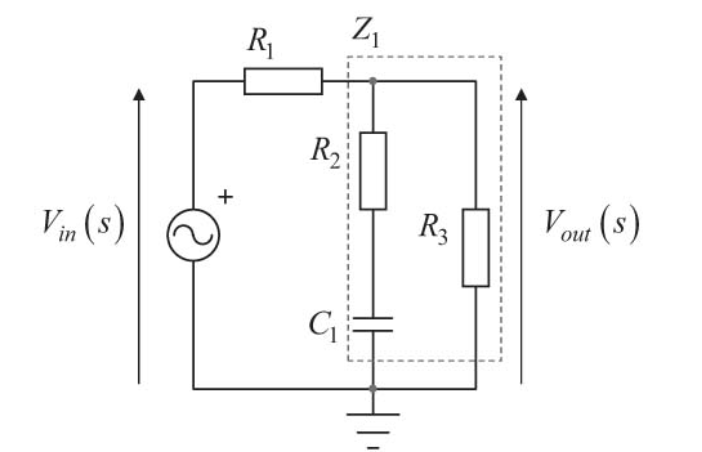
\includegraphics[width=0.5\linewidth]{Z1}
	\caption{Circuito de donde se obtendrá la Z1}
	\label{fig:z1}
\end{figure}
\FloatBarrier

La Z1 será entonces:
\[Zequ=\frac{sLR_{3}+R_3R_2}{R_3+sL+R_2}\]
Teniendo esto se hace un divisor de voltaje para encontrar el voltaje de salida, el cual queda de la forma:
\[V_o=V_{in}\frac{Z1}{Z1+R_1}\]
sustituyendo:
\[V_o=V_{in}\frac{\frac{sLR_{3}+R_3R_2}{R_3+sL+R_2}}{\frac{sLR_{3}+R_3R_2}{R_3+sL+R_2}+R_1}\]
Como lo que se busca el sa función de transferencia se deja fuera $\frac{V_o}{V_{in}}$ y la función queda:
\[\frac{V_o}{V_{in}}=\frac{\frac{sLR_{3}+R_3R_2}{R_3+sL+R_2}}{\frac{sLR_{3}+R_3R_2+R_3R_1+R1sL+R_1R_2}{R_3+sL+R_2}}\]
Por ley de la herradura cancelamos los denominadores para dejarla de la forma:
\[\frac{V_o}{V_{in}}=\frac{sLR_{3}+R_3R_2}{sLR_{3}+R_3R_2+R_3R_1+R1sL+R_1R_2}\]
Agrupando en el denominador:
\[\frac{V_o}{V_{in}}=\frac{sLR_{3}+R_3R_2}{R_3R_2+R_3R_1+R_1R_2+sLR_3+R_1sL}\]
Factorizamos la $R_3$ y la $R_2$ del numerador para dejarlo de la forma que se espera obtener
\[\frac{V_o}{V_{in}}=\frac{R_{3}R_2(\frac{sL}{R_2}+1)}{R_3R_2+R_3R_1+R_1R_2+sLR_3+R_1sL}\]
-una vez hecho esto factorizamos el denominador separando la parte que contiene $sL$ del resto del denominador:
\[\frac{V_o}{V_{in}}=\frac{R_{3}R_2(\frac{sL}{R_2}+1)}{R_3R_2+R_3R_1+R_1R_2(\frac{sL(R_3+R_1)}{R_3R_2+R_3R_1+R_1R_2}+1)}\]
Como lo que se busca es obtener una expresión con resistencias en paralelo, esperamos obtener fracciones como la mostrada en la Ecuación \ref{eq:1}
\begin{equation}
\frac{R_xR_y}{R_x+R_y}
\label{eq:1}
\end{equation}
por lo que hacemos las factorizaciones necesarias para lograrlo.
\[\frac{V_o}{V_{in}}=\frac{R_{3}R_2(\frac{sL}{R_2}+1)}{R_3+R_2(R_1+\frac{R_2R_3}{R_2+R_3})(\frac{sL(R_3+R_1)}{R_3R_2+R_3R_1+R_1R_2}+1)}\]
lo mismo se hace con la otra parte del denominador para dejarlo como:
\[\frac{V_o}{V_{in}}=\frac{R_{3}R_2(\frac{sL}{R_2}+1)}{R_3+R_2(R_1+\frac{R_2R_3}{R_2+R_3})(\frac{sL}{R_2+\frac{R_1R_3}{R_1+R_3}}+1)}\]
Finalmente donde se encuentran las fracciones parecidas a la mostrada en la Ecuación  \ref{eq:1}
\[\frac{V_o}{V_{in}}=\frac{R_{3}//R_2(\frac{sL}{R_2}+1)}{(R_1+R_2//R_3)(\frac{sL}{R_2+R_1//R_3}+1)}\]
La cual ya es nuestra función de transferencia idéntica a la obtenida por el metodo de inspección y que posteriormente se introducirá al software \texttt{scilab} para obtener la gráfica de la respuesta en modo estable del inductor usado en la práctica.\\

Lo primero que tenemos que hacer para introducir nuestra función de transferencia a nuestro programa desarrollado en Scilab es sustituir todos los valores de las resistencias y del inductor, lo cual nos queda de la siguiente forma:\\

$R1=10k$\\
$R2=3.3k$\\
$R3=10k$\\
\[H(s)=\frac{3.3k||10k}{10k+(3.3k||10k)}*\frac{(1+\frac{S(6.77mH)}{3.3K})}{1+\frac{S(6.77mH)}{(10k||3.3k)+3.3k}}\]
Simplificando la ecuación nos queda así:
\[H(s)=\frac{0.1987+S(407.63e-9)}{1+S(1.171e-6)}\]
La forma de la función de transferencia para la cual habíamos realizado el código en Scilab era de la siguiente forma:
\[Y(s)=\frac{1}{S}(\frac{bs+c}{a+sd})\]
Como se puede apreciar la función de transferencia que obtuvimos en este circuito tiene la misma forma que la del programa de Scilab, por lo que los valores de a, b, c y d se encuentran de forma directa.
\lstinputlisting[label={lst:func},caption={Código para generar la gráfica de la respuesta del circuito.}]{pract1.sci} 
\begin{figure}[h!]
	\centering
	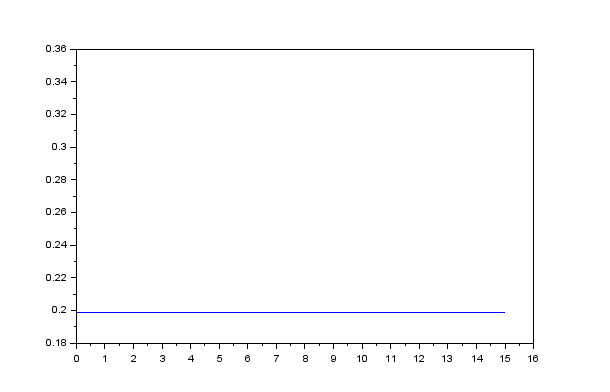
\includegraphics[width=0.5\linewidth]{grafica_programa}
	\caption{Gráfica de la respuesta estable del sistema obtenido de la función de transferencia del circuito}
	\label{fig:graficaprograma}
\end{figure}
\FloatBarrier
\subsection{Parte 2} 
\textbullet Observar la respuesta en el tiempo del circuito en el simulador LTI Spice.
\begin{figure}[h!]
	\centering
	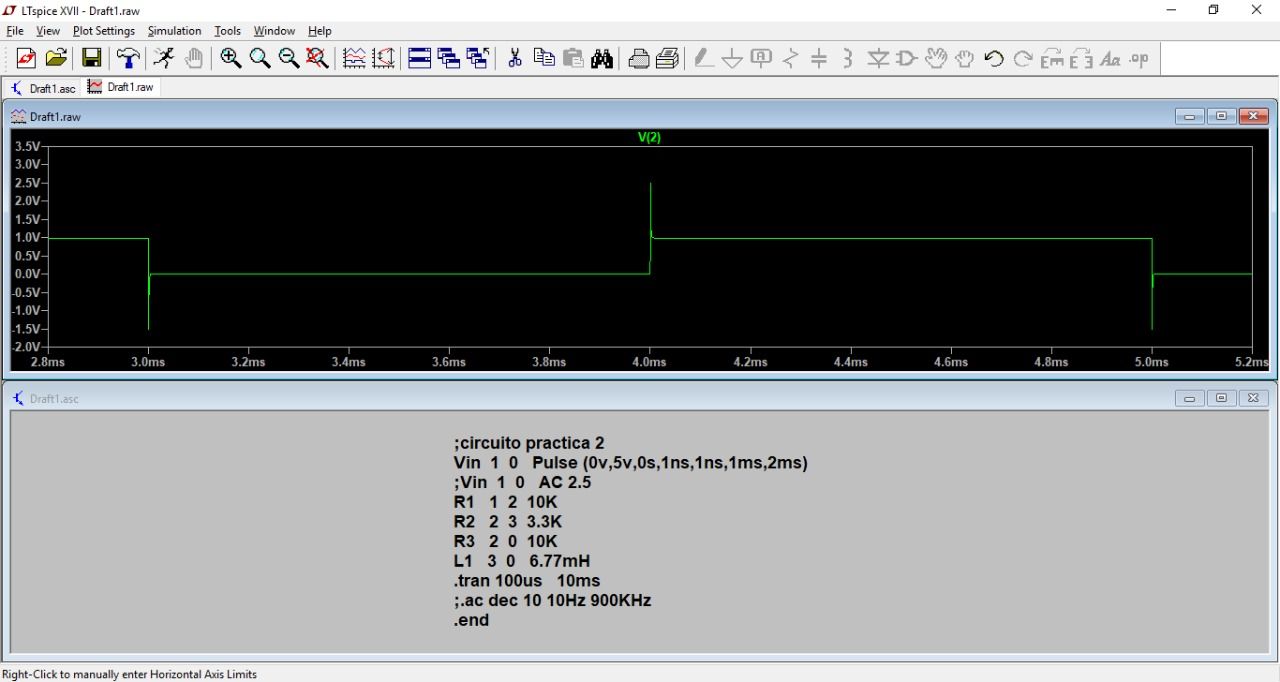
\includegraphics[width=0.8\linewidth]{respuesta_en_escalon_1}
	\caption{Captura de la respuesta en el tiempo del circuito}
	\label{fig:respuestaenescalon1}
\end{figure}
\FloatBarrier
\begin{figure}[h!]
	\centering
	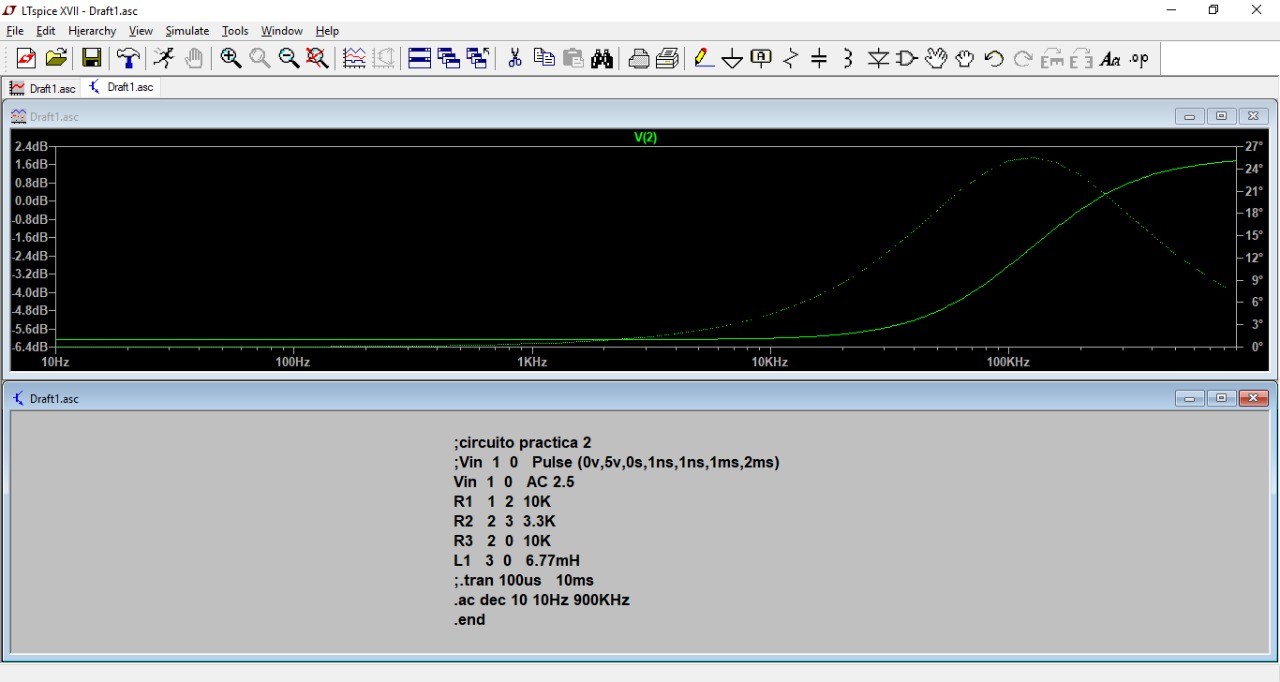
\includegraphics[width=0.8\linewidth]{Bode_sim}
	\caption{Captura de la respuesta en la frecuencia del circuito}
	\label{fig:bode}
\end{figure}
\FloatBarrier
\section{Resultados}
Para la implementación del circuito utilizamos los valores de resistencias y del inductor utilizados en la simulación en Spice, con el generador de señales alimentamos a la entrada con $5V_{pp}$ a $1kHz$ de frecuencia desde donde comenzamos a hacer el barrido de frecuencias para observar su respuesta al variar la frecuencia.
\begin{center}
	\begin{tabular}{|c|c|}
	\hline 
	Frecuencia (Hz) &  $V_{pp}$ (V) \\ 
	\hline 
	1000 & 1.2 \\ 
	\hline 
	10000 & 1.8 \\ 
	\hline 
	20000 & 1.10 \\ 
	\hline 
	30000 & 1.14 \\ 
	\hline 
	40000 & 1.20 \\ 
	\hline 
	50000 & 1.26 \\ 
	\hline 
	60000 & 1.34 \\ 
	\hline 
	70000 & 1.42 \\ 
	\hline 
	80000 & 1.52 \\ 
	\hline 
	90000 & 1.64 \\ 
	\hline 
	100000 & 1.72 \\ 
	\hline 
	200000 & 1.94 \\ 
	\hline 
	300000 & 1.32 \\ 
	\hline 
	400000 & 1.02 \\ 
	\hline 
	500000 & 860e-3 \\ 
	\hline 
	600000 & 760e-3 \\ 
	\hline 
	700000 & 680e-3 \\ 
	\hline 
	800000 & 640-3 \\ 
	\hline 
	900000 & 600e-3 \\ 
	\hline 
\end{tabular} 
\end{center}
La tabla anterior son los resultados que obtuvimos al hacer el barrido en frecuencia yy medir el voltaje de salida.
\begin{figure}[h!]
	\centering
	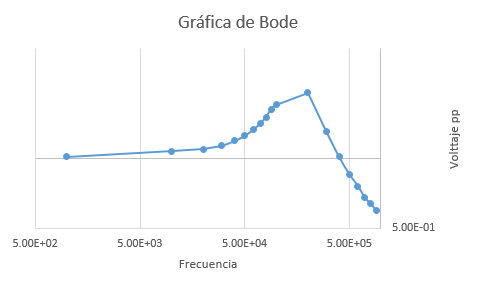
\includegraphics[width=0.7\linewidth]{bode}
	\caption{Gráfica de Bode obtenida con los puntos del barrido de frecuencias}
	\label{fig:bode}
\end{figure}
\FloatBarrier
Otro parámetro importante para calcular es el $\tau$ el cual para el inductor está dado de la siguiente forma:
\[\tau =\frac{L}{R}\]
\[\tau =\frac{6.77mH}{8.3k}\]
\[\tau =815.66ns\]
\begin{figure}[h!]
	\centering
	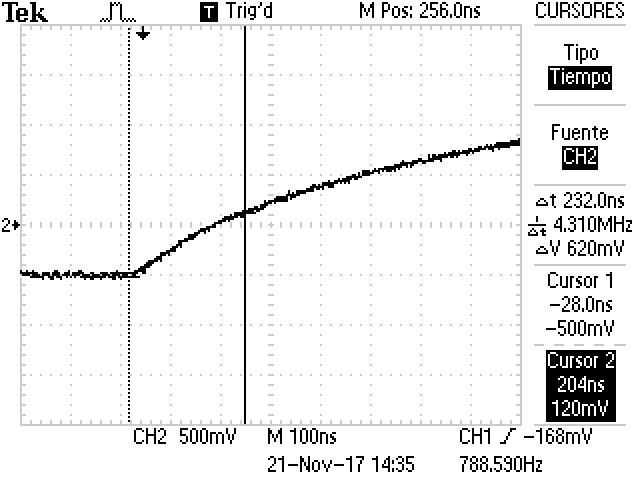
\includegraphics[width=0.5\linewidth]{foto2}
	\caption{Medición de $\tau$ en el inductor donde $\tau=232ns$}
	\label{fig:foto2}
\end{figure}
\FloatBarrier
\section{Conclusiones}
\textbf{José Eduardo Contreras Sandoval}\\
Para poder obtener la respuesta de un sistema o que en este caso fue de un circuito es muy importante poder identificar los ceros y los polos ya que facilitan mucho el trabajo analítico al realizarlo por el método de inspección, el simulador de Spice nos sirvió mucho para que al momento de realizar la implementación física del circuito tuvieramos una idea de que era lo que debíamos esperar en la respuesta de nuestro circuito.\\

A diferencia de la simulación, nuestro circuito a frecuencias superiores a $200kHz$ no se mantenía estable como si lo hacía en la simulación, esto debido a que el inductor utilizado era de núcleo de aire, lo cual para este tipo de inductores sabemos que su frecuencia de trabajo no es muy alta provocando esos comportamientos inesperados en la gráfica de Bode.\\

\textbf{Jorge Alberto Ochoa López}\\
Como conclusión de esta practica puedo decir que al inicio no era algo muy claro de hacer pues 
no se veía muy simple pero paso a paso las coas se fueron aclarando, después de utilizar el inductor y el capacitor de forma practica en el laboratorio,
todo en cuanto a la practica se simplifico un poco pues ya se podía observar físicamente el comportamiento
que se buscaba mediante las ecuaciones planteadas. \\
fue un poco complicado llegar a la misma función de transferencia por ambos métodos pues para saber a que funcion debia llegarse se debía tener ya uno
de los métodos resueltos, lo que costó un poco de tiempo, finalmente cuando ya se tuvieron los resultados de la función de transferencia por ambos métodos y que se introdujo 
en el software \texttt{scilab} con los valores de resistencia e inductancia calculados prácticamente, fue aun mas claro lo que se buscaba pues la respuesta gráfica que nos entrego este software así como 
la gráfica que mostró el simulador LTSPICE fue la misma y pudimos corroborar que las ecuaciones son las correctas.
\end{document}	
	
